\section{Analysis and Case Study}
We used Omnet++ as a simulation tool to explore the most 
suitable model and algorithm for ThinkTogether. The study done by 
Varga~\cite{A_OMNET_ESM01} 
provides brief introduction of Omnet++, including Model Libraries, NED 
language, 
model structure. The paper also describes how to execute the simulation under a 
powerful graphical user interface, which will help the team to better utilize 
the tool. Work done by Anggadjaja et al.~\cite{EI_OMNET_ACT10}. features the 
use of Omnet++ based 
simulation for reliable point-to-point wireless transmission. The outcome could 
provide inspiration for employing P2P model in wireless network. There 
are several other papers~\cite{MM_OMNET_OMN08,XX_OMNET_ICQ12} explaining the 
main infrastructure and 
internal 
design of Omnet++. 
%The team can gain overall understanding of the tool, through 
%extensive papers above, and use Omnet++ with efficiency and accuracy. 

%Experimental data is the most scientific and objective way of verifying the 
efficiency of a particular network. There comes the simulation. 
In our work, 
two network models will be built in order to observe the behavior of data 
packets transferred in between. One of networking protocol is Telnet, on which 
J. Postel et al~\cite{JJ_TEL83} provides specification and 
standard. This is 
a relatively old paper that is published in early 1980s. The paper draws a 
whole picture of telnet protocol from general consideration to signal 
processing. The team refers to this paper to get a understanding of how Telnet 
protocol is put to use. Another protocol adopted is HTTP. There are wider range 
of papers dedicated to HTTP. One done by R Fielding~\cite{BJJH_HTTP1999} 
provides a full-scaled overview, which is used as a reference for modelling. 

%Multilayer Transmission

ThinkTogether is a communication application that contains multiple layers in 
packet transmission. Data sent by each individual is handled differently. G. 
Sekin et al~\cite{GF_COM00} provides an insight of how to manage multi 
priority traffic in ATM network. The study is content-based video 
objects. As the common characteristics shared between video stream and voice 
stream, such as low tolerance in delay, jitter and packet misorder, our team 
could adopt ideas proposed in the paper. Unfortunately, there is no evaluation 
involved in the paper, therefore the feasibility of proposed algorithm remains 
unknown. 


After designing the model, we plan to create a working 
network by creating a simulation using Omnet++, as shown in Fig.~\ref{fig:sce}. 
By creating 
this simulation we can have an idea of how the voice stream packets are being 
transferred between the different nodes present in the network. Once the 
simulation starts working for a basic scenario of just 2 leaf nodes, a relayer 
\& a cloud server, we will add more number of nodes to the simulation and then 
analyse what changes are to be made to certain parameters of the network so as 
to avoid any kind of latency and disturbance while transferring the voice 
streams. 

Presenters initialize services by sending voice packets to both relayers and 
cloud. Upon receiving the packets, the server stores them 
locally and echoes back an acknowledgement. The services between presenter and 
server is now finished. In other side,
voice packets reach the relayer and will be directed to all attendees relayer 
connects to, which is illustrated by \#6 and \#7 event in Fig.~\ref{fig:r_seq}. 
Out of 
testing purpose, each attendees request the exact same voice data from cloud. 
Cloud handles that request by fetching corresponding data in server and sending 
back the requested content. One can refer to events from \#11 to \#16 for 
execution sequence details. 
 

 
\section{Implementation: Data Distribution and Layers}

The simulation tests the efficiency in transferring voice data packets 
with a fundamental model. This model lays the groundwork for future expansion, 
and illustrates a simple way to consider a classroom scenario. The purpose of 
simulation is 
to investigate the feasibility, and more importantly, the efficiency of the 
model. In the simulation, parameters such as packet drops, delay time, etc. are 
collected and extracted to generate an output file for further analysis. The 
output file is then used as 
a foundation for performance analysis.  


%In this paper our aim is to deploy a distributed the feature of voice 
%streaming in the 
%already developed application of Two Tall Totems called Think Together. In 
%order to implement this feature we have 
In our simulation of the model architecture, we use multiple nodes 
as the leaf nodes in a network. 
Then we also have some nodes that act as relayers in the network that will 
transfer the voice stream from the presenter in the network to 
the corresponding leaf nodes in the network. Along with all these nodes we also 
have a cloud server which will act as a primary storage device for all the 
voice streams that will transmitted throughout the network. All the nodes will 
have a direct link to the server so that if any of the leaf nodes (student 
nodes in our scenario) wants to retrieve any voice stream they can do so by 
making a request to 
the cloud server for that voice stream directly through the relayer (big node). 

To simplify, we assume all the attendees are physically located in the same 
classroom and they are subscribing to voice for the purposes of capturing the 
information. This will eliminate potential influence caused by the difference 
of 
location, such as propagation delay. There are five components in the model: 
presenter, relayer, cloud, server and attendee. Each component coordinates with 
one another in order to offer recording services to attendees. There are two 
test cases, one as a small-scaled network with two attendees, the other as 
slightly larger-scaled network with ten attendees. The simulation 
is run in HTTP net, 
masking the lower level network layers such as TCP and IP. 


%Model Taxonomy

Figure~\ref{fig:sce} shows the overall picture of the simulation model in 
small-scaled case. It 
breaks down to four  parts: sender (presenter), receiver (attendees), 
mediator (relayers), and backup (cloud and server). 

\begin{figure}[h!]  
  \centering
    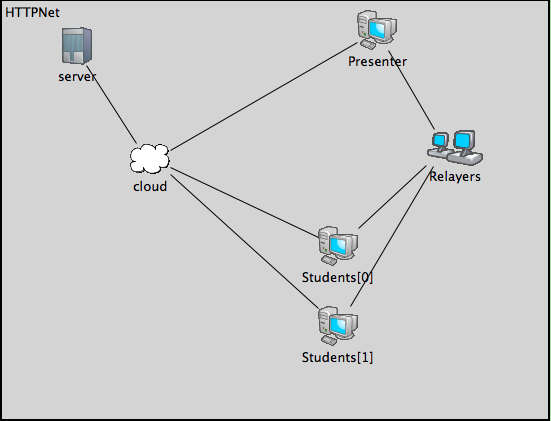
\includegraphics[width=0.5\textwidth]{figures/sce.png}
  \caption{Simulation in Omnet++}
  \label{fig:sce}
\end{figure}

Presenter is the starting point of service. It does not rely on any outer 
resource to trigger sending process. Currently no packets other than 
acknowledgement are sent to presenters. In other words, one can view presenters 
as a resource provider and there is no prerequisite for presenters to function. 
There are two outgoing links connected to presenters. The one connected to 
relayers is the main channel for delivering data. The one connected to cloud 
transfers the same content, yet it is less demanding in terms of propagation 
speed and processing time. A presenter sends voice packets to both links 
simultaneously, and sets a timer for next cycle. 

The cloud server can be considered as a group in terms of services 
purpose. 
They 
are both built to provide backup for attendees. There are two scenarios in 
which 
attendees would need backup services. The first is when packets are lost by the 
relayers and attendees will ask for complementary data from cloud to ensure a 
smooth stream. The second is when attendees are not able to attend 
the 
class, but request a later review of that class. The server stores the 
lectures in the format of voice stream and delivers it to attendees via cloud. 
In this regard, the cloud is an interface between service providers and 
receivers. In addition, once network is scaled up to include multiple servers, 
cloud acts as coordinator that organizes servers’ actions. 

The relayer acts as a router in this simple case simulation. Unlike servers, 
the relayer 
does 
not store voice data, thereforegull attendees can not request data from relayer 
later on. It should be noted that this primary function is not yet implemented, 
and will be 
addressed later in future model. 

Attendees are students in the diagram. They receive voice packets from 
presenters, regularly through relayers. It should be noted that attendees will 
not send 
acknowledgement back to presenters. When the network between relayers and 
attendees are down, or for some reason, packets are lost in the regular 
transmission routes, attendees will request the data from the server. The 
target 
users of ThinkTogether app is attendees and presenters.  
%Execution Sequence:

To collect data from multiple cycles, we set a timer for both presenter and 
attendees based on an exponential distribution. After sending the voice 
packets, 
the presenter will create a timer that controls how long before the next cycle, 
namely, the next time it starts sending the packets. The duration of the timer 
is based on a exponential function, which allows random distribution in sending 
packets. The same principle applies to rate of sending request from attendees. 
There is also a timer created by attendee that controls the rate of sending 
requests to cloud. In real life, an attendee need complementary data from cloud 
only when relayers fail to deliver it. However, in order to fully evaluate the 
function, in the simulation we configure an attendee to request voice data from 
the cloud whether the relayers go down or not.

\begin{figure}[h!]
  \centering
    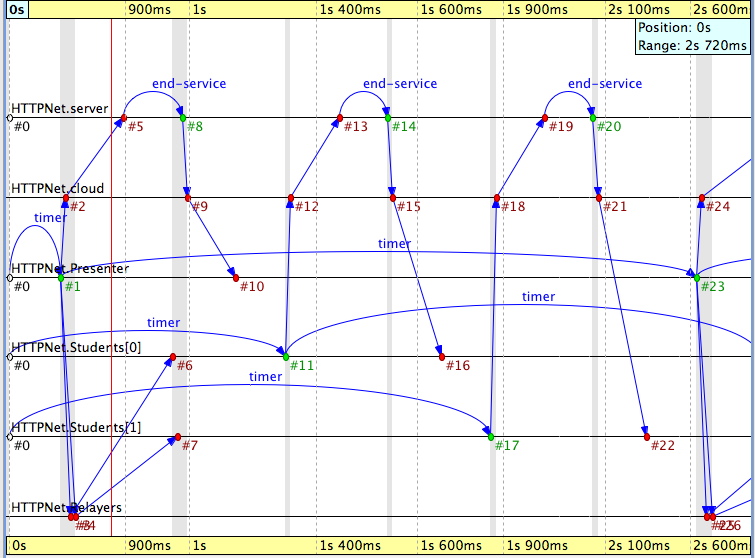
\includegraphics[width=0.5\textwidth]{figures/r_seq.png}
  \caption{Events in Time Sequence}
  \label{fig:r_seq}
\end{figure}

The execution sequence is illustrated by diagram below. It is a log file 
generated by running a small-scaled cases. 

%\section{Deployment: Distributed Cloud}


